\documentclass[12pt]{article}
\usepackage{fancyhdr}     % Enhanced control over headers and footers 
\usepackage[T1]{fontenc}  % Font encoding
\usepackage{mathptmx}     % Choose Times font 
\usepackage{microtype}    % Improves line breaks      
\usepackage{setspace}     % Makes the document look like horse manure 
\usepackage{hyperref}
\hypersetup{
	colorlinks   = true, %Colours links instead of ugly boxes
	urlcolor     = blue, %Colour for external hyperlinks
	linkcolor    = black, %Colour of internal links
	citecolor   = black %Colour of citations
}
\usepackage{graphicx}
\usepackage{subcaption}
\usepackage{endnotes}
\usepackage{float}
\usepackage{algorithm}
\usepackage{algpseudocode}
\usepackage{multicol}
\usepackage{tikz}
\usetikzlibrary{snakes}
\usepackage{rotating}
\usetikzlibrary{positioning,shapes.multipart}
 \usepackage{listings}

\usepackage[style=apa,backend=biber,citestyle=numeric]{biblatex}
\addbibresource{../refs.bib}

\title{Bayesian Neural Networks}
\author{
	Blair, Taylor
	\and
	Sorgmon, Ava
	\and
	Conor
}
\date{\today}
\let\footnote=\endnote

\usepackage{verbatim}

\pagestyle{fancy} % Default page style 
\lhead{Blair, Sorgman, Conor}
\chead{}
\rhead{\thepage}
\cfoot{}
\rfoot{}
\renewcommand{\headrulewidth}{1pt}
\renewcommand{\footrulewidth}{1pt}
\renewcommand{\theendnote}{\Roman{endnote}} 



\begin{document}
\doublespacing
\maketitle



\begin{abstract}
	Bayesian Neural Networks are...
\end{abstract}

\tableofcontents

\section{Introduction}

	
\section{Machine Learning}
	
% To understand the concept of deep learning, we first need to understand the broader area it is considered a subset of; machine learning. 
%Machine learning is considered to be a branch of artificial intelligence (AI) with the goal to help AI “learn” more, but specifically in a way that imitates the human process of learning through the use of data and algorithms\cite{ibmWhatIsML}. 
Machine learning includes a variety of topics of which artifical intelligence (AI) and neural networks are a subset. Neural networks in particular involve an abstract imitation of the human brain using simulated neurons which is trained on data using particular algorithms. 

The term supervised learning refers to a specific common method of machine learning which uses a labeled dataset to train a model to correctly predict the labels via some training algorithm. A classification problem in supervised learning involves predictions where all labels are grouped into a set of categories. The training process can be broken down into three major steps, which include a decision process, an error function, and an optimization process \cite{berkelyWhatIsML}. The decision process is the set of steps the algorithm takes after receiving the data based on the goal of the model. The second step in the process is the error function, which is the method of measuring chosen to see if the algorithm gave a “good” or “bad” input. The two most common choices of the error function is a simple yes or no on if a data point was classified correctly in the case of classification, or the difference in value between the predicted outcome and the actual observed outcome for continuous values. Finally, the third and last step is the part of the process that implements learning. This step, the updating or optimization process, requires the algorithm to review the past data and outputs of the error function in order to better correct its decision making process in the future.

Throughout this report, we’ll often use the terms machine learning, deep learning, and neural networks. It is important to note that although these are fundamentally related fields, deep learning is a subfield of neural networks that in particular focuses on more complicated neural networks, while neural networks are a subfield in machine learning. 

We will be training a classifier on labeled images in a supervised learning process to predict what is depicted in the image from a range of possibilities such as dog, cat, and plane.


% EDIT THIS SECTION But, back to deep learning! What sets deep learning apart from the more general machine learning is that unlike the supervised learning process that was described before, deep learning does not necessarily have to use pre labelled data sets. It can, if required, but the point of a deep learning algorithm is that one feature of the algorithm is that it itself can distinguish between the different types of data purely by looking at the data. This process of built in categorical distinction is extremely helpful, as it limits human interaction and interventions that are required in the learning process, as large amounts of data do not need to be “processed by hand” in order for the algorithm to make use of them (2). Deep learning models work through a “layering” process, where multiple layers of the original three steps listed above work together in the algorithmic process.

	
\subsection{Neural Network}

\begin{figure}[H]
	\centering
	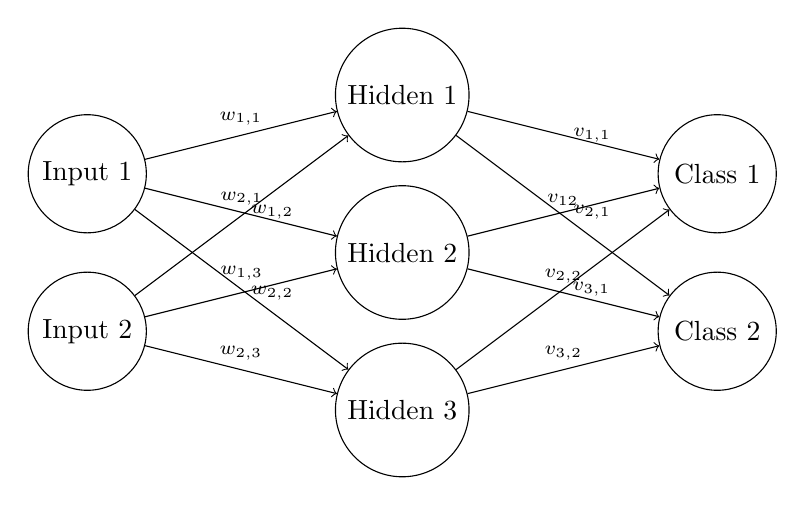
\begin{tikzpicture}
		% Define node styles
		\tikzstyle{neuron} = [circle, draw, minimum size=1.5cm];
		\tikzstyle{weight} = [font=\scriptsize];
		
		% Input layer (2 neurons)
		\node[neuron] (input1) at (-2,1) {Input 1};
		\node[neuron] (input2) at (-2,-1) {Input 2};
		
		% Hidden layer (3 neurons)
		\node[neuron] (hidden1) at (2,2) {Hidden 1};
		\node[neuron] (hidden2) at (2,0) {Hidden 2};
		\node[neuron] (hidden3) at (2,-2) {Hidden 3};
		
		% Output layer (2 neurons for classification)
		\node[neuron] (output1) at (6,1) {Class 1};
		\node[neuron] (output2) at (6,-1) {Class 2};
		
		% Connections with weights
		\draw[->] (input1) -- node[weight, above] {$w_{1,1}$} (hidden1);
		\draw[->] (input2) -- node[weight, above] {$w_{2,1}$} (hidden1);
		\draw[->] (input1) -- node[weight, right] {$w_{1,2}$} (hidden2);
		\draw[->] (input2) -- node[weight, right] {$w_{2,2}$} (hidden2);
		\draw[->] (input1) -- node[weight, above] {$w_{1,3}$} (hidden3);
		\draw[->] (input2) -- node[weight, above] {$w_{2,3}$} (hidden3);
		\draw[->] (hidden1) -- node[weight, right] {$v_{1,1}$} (output1);
		\draw[->] (hidden2) -- node[weight, right] {$v_{2,1}$} (output1);
		\draw[->] (hidden3) -- node[weight, right] {$v_{3,1}$} (output1);
		\draw[->] (hidden1) -- node[weight, above] {$v_{12}$} (output2);
		\draw[->] (hidden2) -- node[weight, above] {$v_{2,2}$} (output2);
		\draw[->] (hidden3) -- node[weight, above] {$v_{3,2}$} (output2);
	\end{tikzpicture}
	\caption{Example neural network}
	\label{fig:example-nn}
\end{figure}

A neural network takes a series of inputs. An example of a neural network with two inputs, one hidden layer of size three, and two outputs appears in figure \ref{fig:example-nn}  

\subsection{Neural Network Neurons}


\begin{figure}[H]
	\centering
	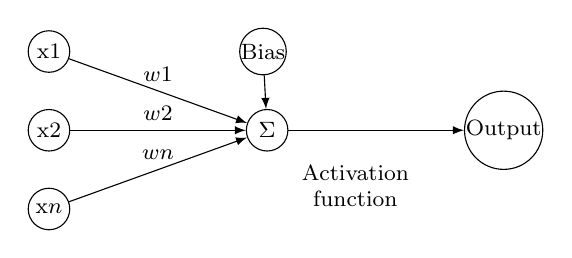
\begin{tikzpicture}[
		neuron/.style={
			circle,
			draw,
			minimum size=1.5em,
			inner sep=0pt,
		},
		font=\footnotesize,
		>=latex
		]
		% Draw the neuron
		\node [neuron] (neuron) at (0,0) {$\Sigma$};
		% Draw the input nodes and labels
		\foreach \i/\txt in {1/$1$,2/$2$,3/$n$} {
			\node [neuron,left=of neuron] (input\i) at (-1.5,-\i +2) {x\txt};
			\draw[->] (input\i) -- node[above] {$w$\txt} (neuron);
		}
		% Draw the bias node and label
		\node [neuron,left=of neuron] (bias) at (1.25,1) {Bias};
		\draw[->] (bias) -- node[right] {} (neuron);
		% Draw the activation function label
		\node[align=center,below right =0.5em of neuron] {Activation \\ function};
		% Draw the output node and label
		\node [neuron,right=of neuron] (output) at (1.5,0) {Output};
		\draw[->] (neuron) -- node[above] {} (output);
		% Draw the relevant functions
		%\draw[->] (0,-1.5) -- (0,-2.5) node[midway,right] {Weighted sum};
		%\draw[->] (-1.5,-3.5) -- (-1.5,-4.5) node[midway,left] {Bias};
		%\draw[->] (1.5,-0.5) -- (1.5,-1.5) node[midway,right] {Activation};
		
		% Draw the activation function shape
		%\node[draw,rectangle,minimum width=2em,minimum height=2em] (actfunc) at (0,1) {};
		%\node[above=0.1em of actfunc] {ReLU};
		
	\end{tikzpicture}
	\caption{Neural network neuron}
	\label{fig:neuron}
\end{figure}

Neural networks are made out of a series of neurons... The neurons take a set of inputs, multiplies the inputs by the weights, sums the weighted input, adds a bias, and runs the output through an activation function...

\subsection{Convolutional Neural Networks }

\begin{figure}[H]
	\centering
	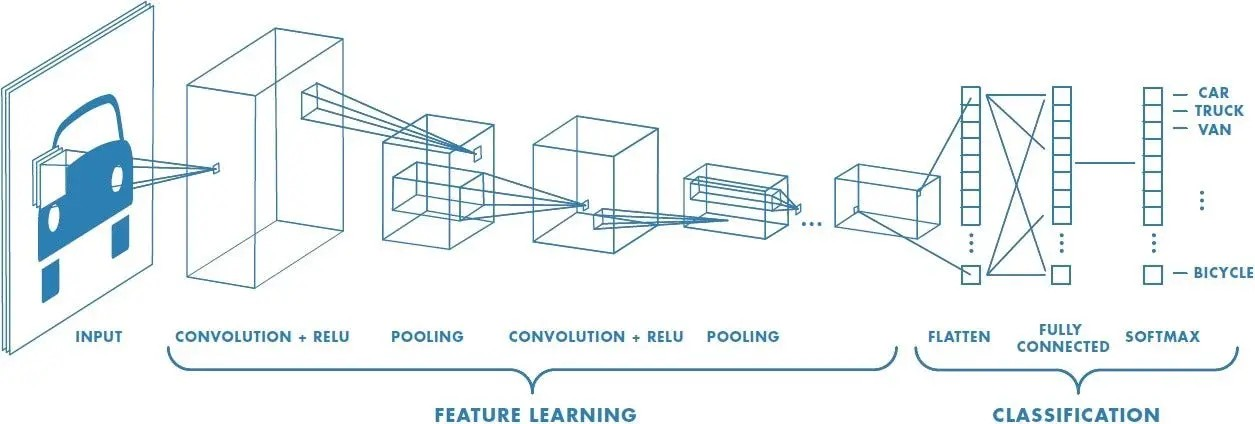
\includegraphics[width=.8\textwidth]{../Images/big-pic-cnn.jpg}
	\caption{CNN pipeline \cite{eli5CNN}}
	\label{fig:cnn-pipeline}
\end{figure}

Convolutional neural networks (CNN) are a type of neural network that is better suited for image recognition. While this might sound like a seperate model structure, CNNs are largely the same. In figure \ref{fig:cnn-pipeline} the difference between a traditional neural network is the convolutional layer. Instead of reading the entire image at once, a convolutional layer slides over the image...

IMAGE OF SLIDING (gif split)



\section{Bayesian Neural Networks}

\begin{figure}[H]
	\centering
	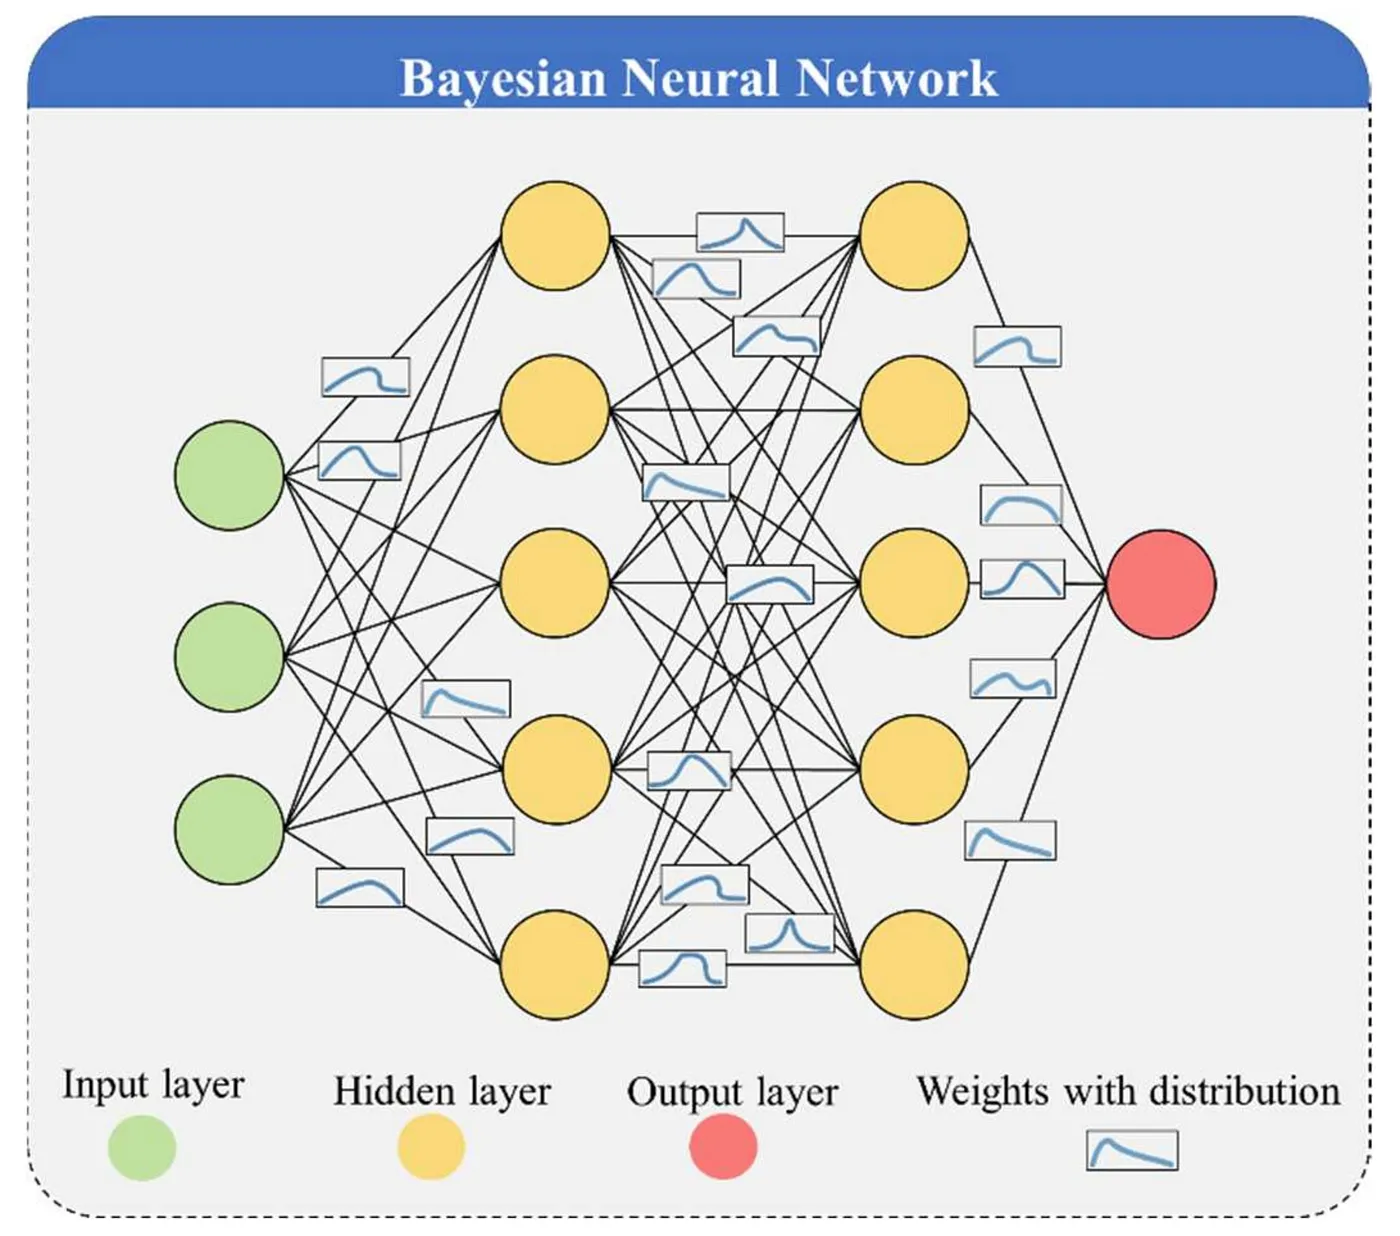
\includegraphics[width=.55\textwidth]{../Images/example_bnn.png}
	\caption{Example BNN  \cite{FleszarBNN}}
\end{figure}

Bayesian neural networks operate the same way as a normal 

\subsection{Bayesian Neural Network Neuron}

Similar to a neural network such as... 

\begin{figure}[H]
	\centering
	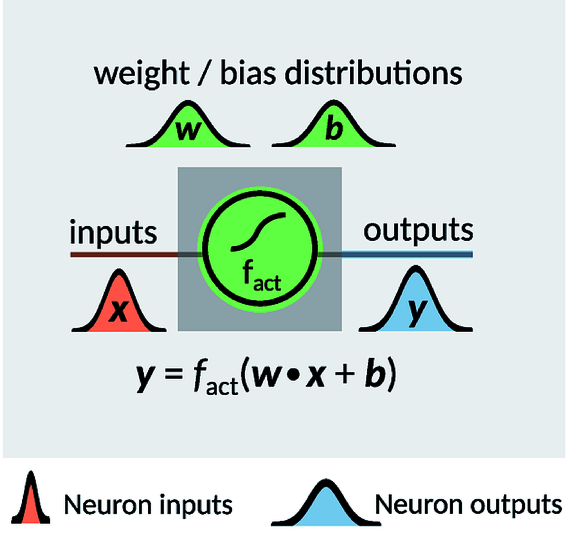
\includegraphics[width=.55\textwidth]{../Images/BNN-neuron.png}
	\caption{Example BNN Neuron \cite{hase2019machine}}
\end{figure}

\subsubsection{Priors}

This section was requested by Micheal. 

\subsection{Bayesian Convolutional Neural Networks}

Bayesian convolutional neural network (BCNN) are similar to CNNs. The difference between is that BCNNs and a CNN is that the BCNN uses a bayesian neuron.

\section{Simulation}

We use a BCNN implementation from \href{https://github.com/kumar-shridhar/PyTorch-BayesianCNN}{Github} based on work from ... \cite{shridhar2019comprehensive} \cite{shridhar2018uncertainty}

\subsection{CIFAR-10}

	\begin{figure}[H]
		\centering
	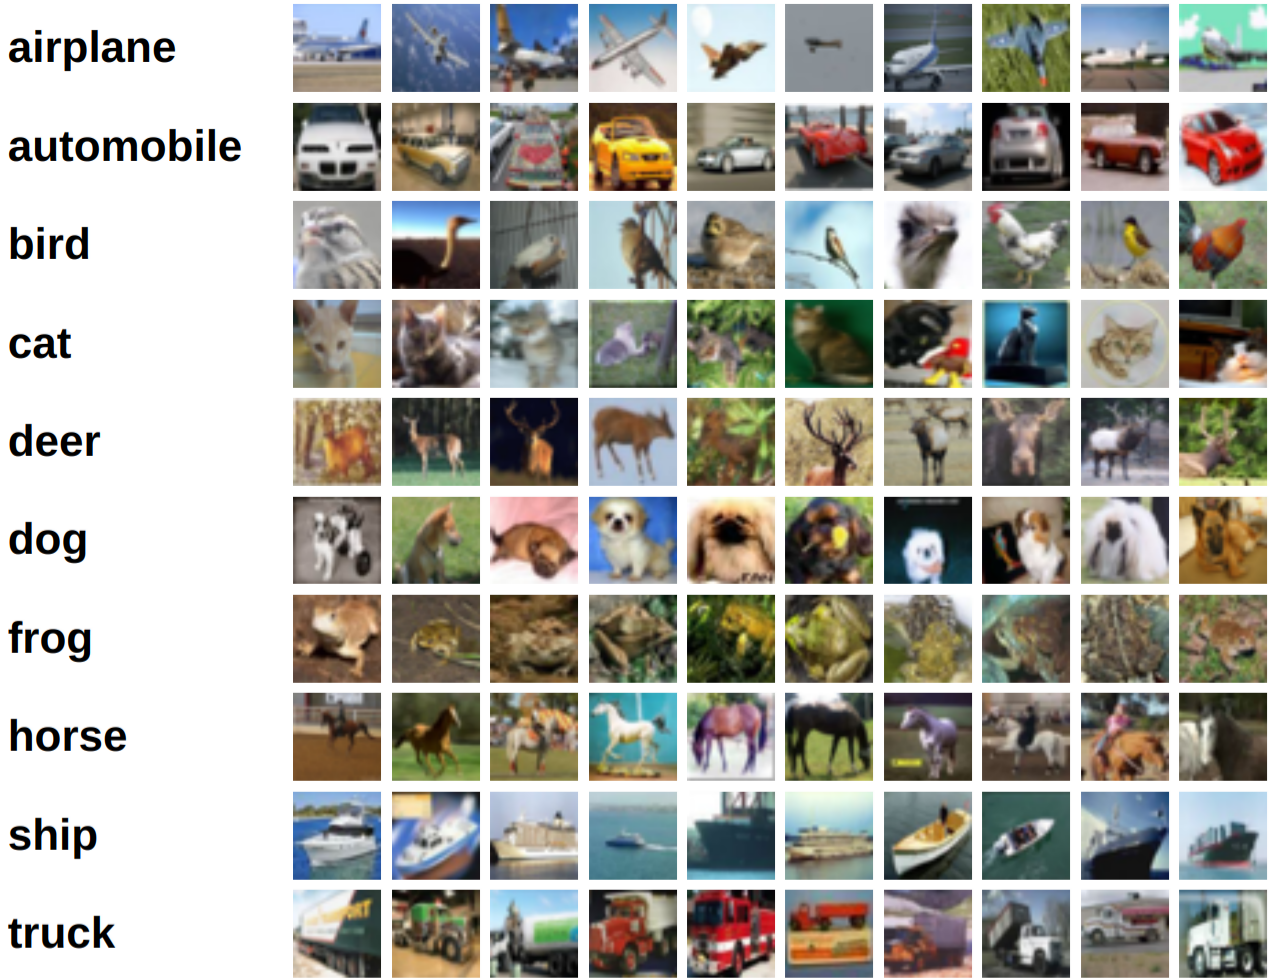
\includegraphics[width=.75\textwidth]{../Images/cifar-10.png}
	\caption{Example CIFAR-10 images \cite{cifar10}}
\end{figure}

The CIFAR-10 ((Canadian Institute For Advanced Research 10) dataset is a popular machine learning  dataset set. It contatins 60,000 $16 \times 16$ color pictures of: airplanes, cars, birds, cats, deer, dogs, frogs, horses, ships, and trucks\cite{cifar10}. Because of its simple task and variety of images, it is often used as a baseline task for new  model structures. 


\subsection{Hyperparamaters}

We used the following hyperparamaters for training:
\begin{figure}[H]
	\begin{center}
	\begin{tabular}{|c||p{3cm}|p{3cm}|} % Adjust p{width} as needed
	\hline
	\textbf{Hyperparameter} & \textbf{CNN} & \textbf{BCNN} \\ [0.5ex] 
	\hline\hline
	Epochs & 100 & 100\\
	\hline
	Learning Rate & 0.001  & 0.003  \\
	\hline
	Regularization Rate& 0.001 & 0.001 \\
	\hline
	Optimizer & Adamw  & Adamw  \\
	\hline
\end{tabular}
\end{center}
\end{figure}


In addition to the hyperparamaters above, the two models have the same number of layers and levels. We did not adjust the priors, as those were set by the BCNN layer code from \cite{shridhar2018uncertainty}. 


\subsection{Results}



\begin{figure}[H]
	\begin{tabular}{|c||p{3cm}|p{3cm}|} % Adjust p{width} as needed
		\hline
		\textbf{Metric} & \textbf{CNN} & \textbf{BCNN} \\ [0.5ex] 
		\hline\hline
		Train Accuracy & 84.96\% & 81.27\%\\
		\hline
		Validation Accuracy & 61.76\%  & 59.21\%  \\
		\hline
		Time to Train & 16 min 11 sec  & 22 min 11 sec  \\
		\hline
	\end{tabular}
\end{figure}


The results we achieved with training were about the same between the BCNN and the CNN. However, the bayesian model took longer to train.

\begin{figure}[H]
	\centering
	\begin{subfigure}{.5\textwidth}
		\centering
		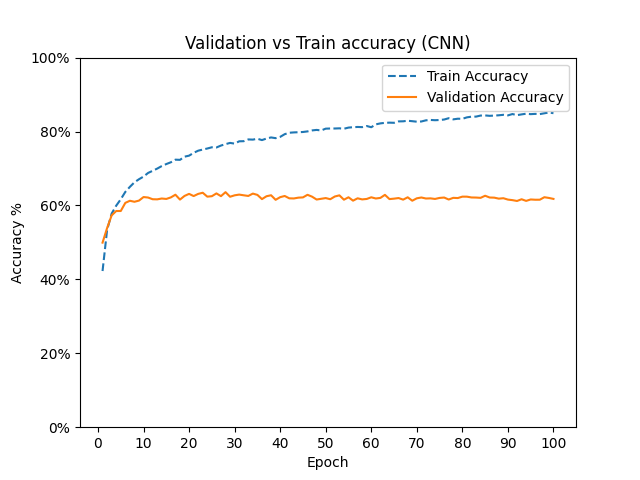
\includegraphics[width=\linewidth]{../Images/CNN_val_acc_over_time}
		\caption{CNN}
	\end{subfigure}% //  
	\begin{subfigure}{.5\textwidth}
		\centering
		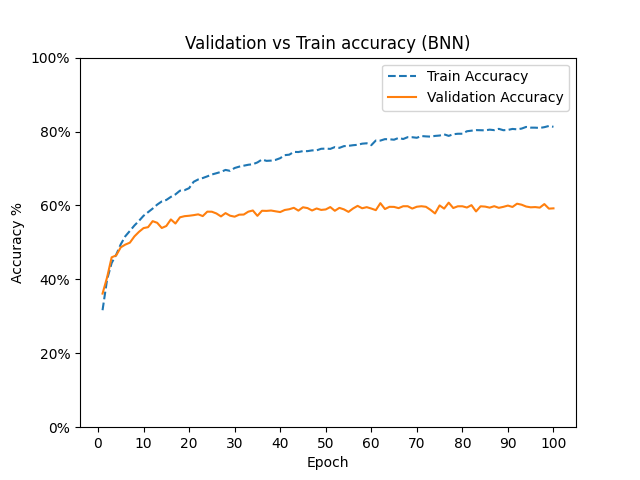
\includegraphics[width=\linewidth]{../Images/BNN_val_acc_over_time}
		\caption{BCNN}
	\end{subfigure}
	\caption{Train vs validation accuracy over time}
	\label{fig:train-v-val}
\end{figure}

Additionally, neither model converged with the train and validation accuracy, this is an indication that we might need to increase the regularization rate. Another thing to note from figure \ref{fig:train-v-val} is that the BCNN took longer to divirge from the train accuracy.

\begin{figure}[H]
	\centering
	\begin{subfigure}{\textwidth}
		\centering
		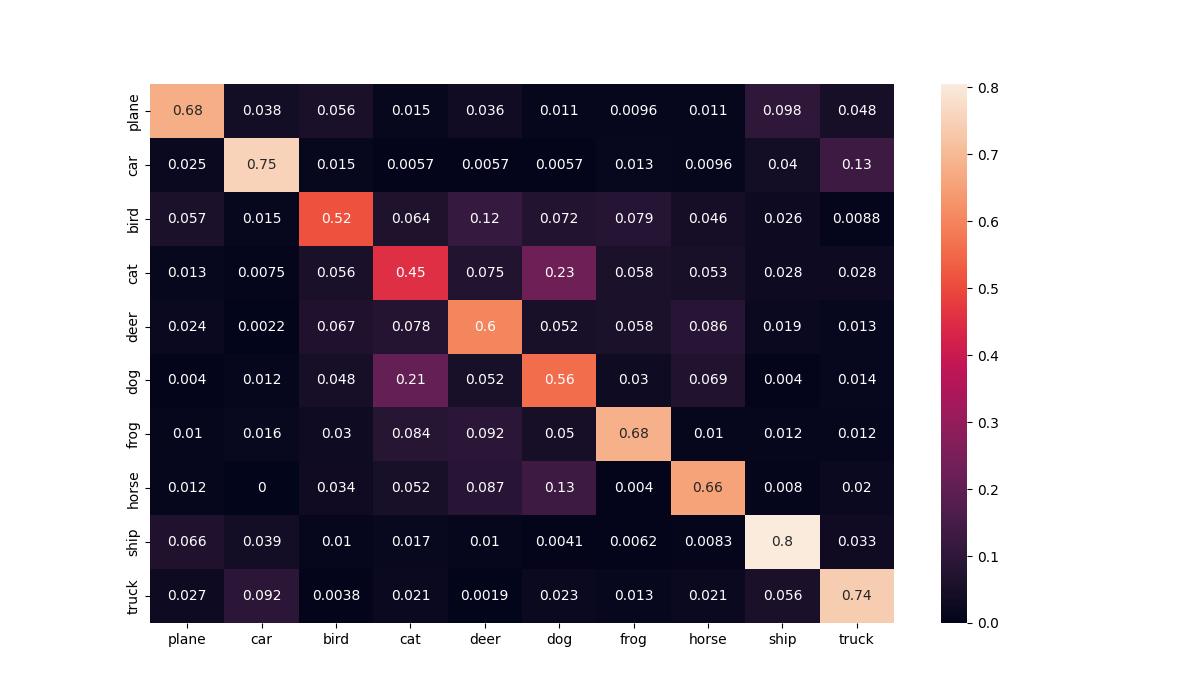
\includegraphics[width=.9\linewidth]{../Images/CNN_confusion_matrix}
		\caption{CNN}
	\end{subfigure} \\% //  
	\begin{subfigure}{\textwidth}
		\centering
		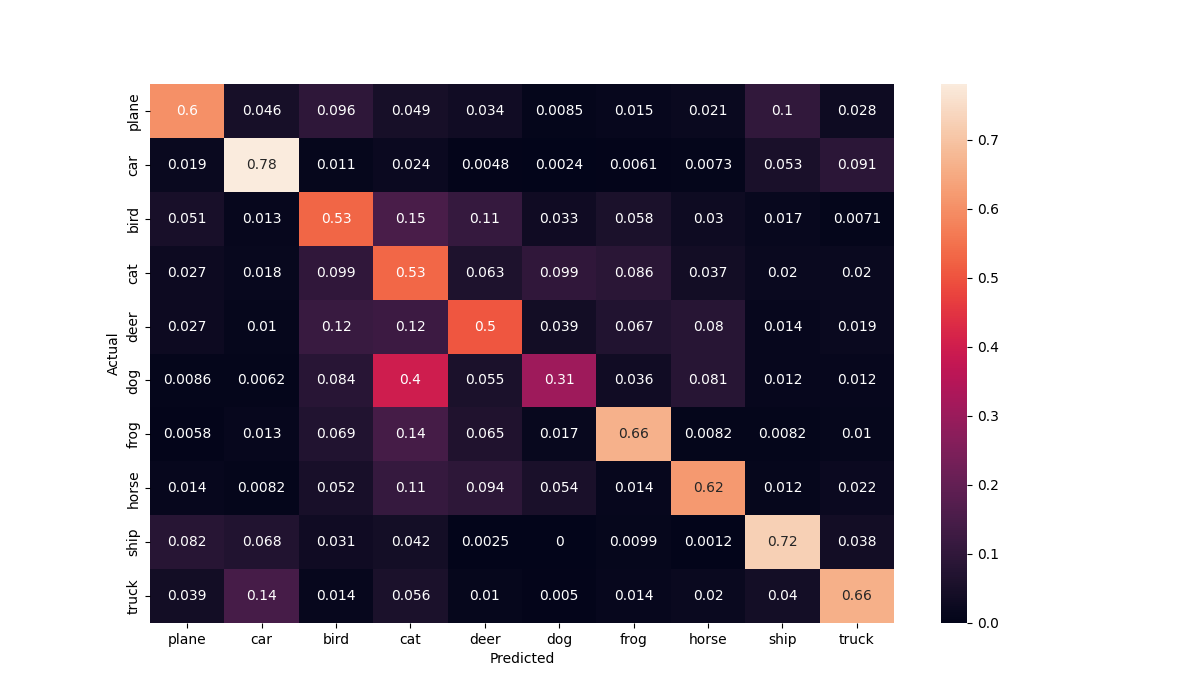
\includegraphics[width=.9\linewidth]{../Images/BNN_confusion_matrix}
		\caption{BCNN}
	\end{subfigure}
	\caption{Confusion matrices}
\end{figure}

The two models have the same set of confusions

\section{Closing}



\newpage

\printbibliography


\end{document}
